\section{Introduction}

In computer architecture, the ``memory wall''~\cite{wulf_mckee_1995}
is a well known problem. Slow memory act as a bottleneck in a system
with fast processors. The reason for this is that processors will
request data faster than what primary memory can provide. In a Von
Neumann architecture\todo{find article to cite here}, the processor
will stall as it waits for the next data or instruction to arrive.

There are several techniques used in modern systems which mitigates
this bottleneck, like caching, outsourcing memory management to a DMA,
branch predictions, etc. One interesting approach is named
``prefetching''.

Prefetching involves speculating in which memory
addresses are needed in the near future, and fetching them prior to
execution. This paper investigates the ``speculating'' part, that is,
what addresses should we fetch and when. When the prefetching is
successful, we avoid CPU stalling as the processor has the needed data
available and we get increased performance. When we are unsuccessful,
we waste valuable cache space.



% \begin{center}
% 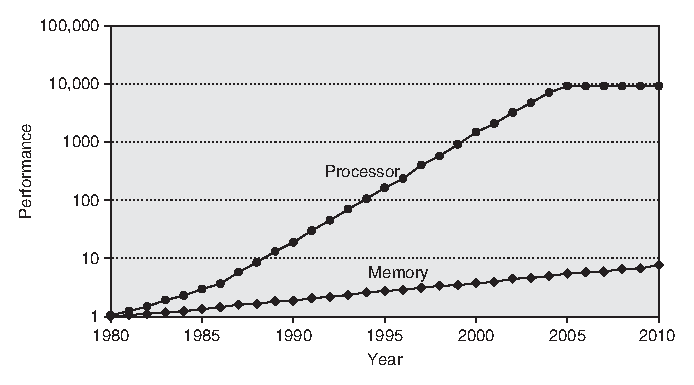
\includegraphics[width=0.5\textwidth]{graphs/memorywall}
% \end{center}

% http://ieeexplore.ieee.org/abstract/document/5389383/




